\documentclass{beamer}

\usepackage{tikz,pgfplots}

\title{Parasites in Structural and Dynamical models of Food Webs}
\author{Nick Kappler}
\date{\today}


\begin{document}
\frame{\titlepage}

\section[Outline]{}
\frame{\tableofcontents}

\section{Motivation}

\begin{frame}
\frametitle{Parasitism in Food Webs}
\begin{itemize}[<+->]
\item  Underrepresented
\item  Novel, complex, and specific
\item  Place in Food Webs
\end{itemize}
\end{frame}

\begin{frame}
\frametitle{Past Work}
\begin{itemize}[<+->]
\item  Adding Parasites to Existing Food Webs%\footnote{\tiny\bibentry{Dunne2013}}
\item  Importance of Body Size Ratios %\footnote{\tiny\bibentry{Brose2006}}
\item  An Inverse Niche Model %\footnote{\tiny\bibentry{Warren2010}}
\end{itemize}
\end{frame}

\begin{frame}
\frametitle{Research Goals}
\begin{itemize}[<+->]
\item Niche Model with Parasites
\item  Dynamical Simulations with Parasites
\end{itemize}
\only<3>{
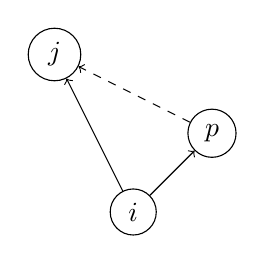
\begin{tikzpicture}
\node[draw,circle] at (0,0) (j) {$j$};
\node[draw,circle] at (1,-2) (i) {$i$};
\node[draw,circle] at (2,-1) (p) {$p$};
\draw[->] (i)--(j);
\draw[->] (i)--(p);
\draw[->,dashed] (p)--(j);
\end{tikzpicture}
}
\end{frame}


\begin{frame}
\frametitle{The Niche Model}
\begin{tikzpicture}
\draw (0,0)--(10,0)
node[anchor = west] {$n$};
\draw (0,.2)--(0,-.2)
node[anchor = north] {$0$};
\draw (10,.2)--(10,-.2)
node[anchor = north] {$1$};
%Predator
\fill (7,0) circle (.07) 
node[anchor = north]  {$n_j$};
%Predator Diet
\draw (7,0)--(7,.75)--(2,.75)--(2,.5);
\draw (.3,0) -- (.3,.5) -- (3.7,.5) -- (3.7,0);
\draw[dashed] (2,.5) -- (2,0) 
node[anchor = south east] {$c_j$};
\draw[<->] (.3,-.5) -- (3.7,-.5)
node[fill=white,pos = 0.5] {$r_j$}; 
\draw[dashed] (.3,0)--(.3,-.55);
\draw[dashed] (3.7,0)--(3.7,-.55);
%Prey
\fill (3,0) circle (.07) 
node[anchor = north west]  {$n_i$};
\draw(4.2,-2) circle (.3)
node {$i$};
\draw[->] (4.5,-2) -- (5.5,-2);
\draw(5.8,-2) circle (.3)
node {$j$};
\end{tikzpicture}
\end{frame}

\subsection{Models}

\begin{frame}
\frametitle{The Allometric Trophic Network (ATN) Model}
***Non Dimensional
\begin{equation}\label{eq:ATNAAAI}
\begin{array}{r l}
\frac{dB_{i}}{dt} &= r_{i}\left(1-\frac{\sum_{j\in \text{basal}}B_{j}}{K}\right)B_{i}\\[1ex]
& - x_{i}B_{i}\\[1ex]
& + x_{i}B_{i}\sum_{j \in \text{diet}(i)}F_{ji}y\\[1ex]
& - \sum_{j \in \text{pred}(i)}x_{j}B_{j}F_{ij}y/e_{ij} \\[1ex]
\end{array}
\end{equation}

and

\begin{equation}\label{eq:FRAAAI}
F_{ij} = \frac{\omega_{ij}B_{i}^{h}}{B_{0}^{h}+ \sum_{k\in \text{diet}(j)}\omega_{kj}B_{k}^{h}}
\end{equation}
\end{frame}

\begin{frame}
\frametitle{Allometry in the ATN}
\begin{itemize}[<+->]
\item A 'middle' road
\item Punchline:
\[
x_i=a_xM_i^{-0.25}
\]
\item i.e. measuring mass vs. attack rates
\end{itemize}
\end{frame}

\subsection{From Structure to Parameters}


\begin{frame}
\frametitle{Allometric Scaling}
\begin{itemize}[<+->]
\item From many parameters, one
\item $x_i = a_xM_i^{-0.25}$
\end{itemize}
\end{frame}

\begin{frame}
\frametitle{Consumer - Resource Body Size Ratio}
\begin{itemize}[<+->]
\item Use trophic levels:
\[
M_i=Z^{TL-1}
\]
\item Defines an 'average' size hierarchy.
\end{itemize}
\end{frame}

\begin{frame}
\frametitle{Body Size Hierarchy}
$Z = 10$ (no parasites):
\only<1>{
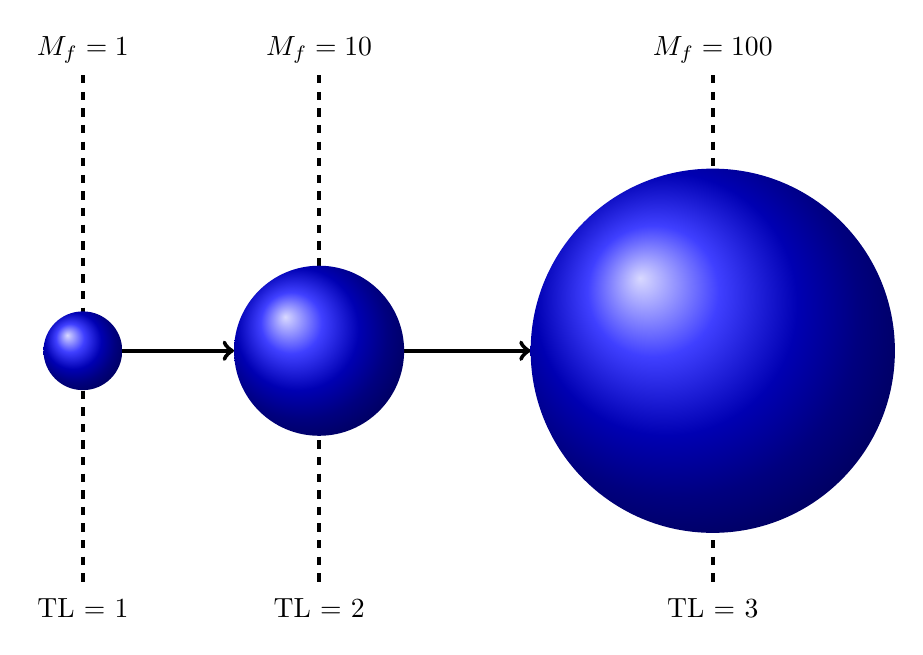
\begin{tikzpicture}
\draw[->,ultra thick] (.5,-1) -> (1.92,-1);
\draw[->,ultra thick] (4.08,-1) -> (5.687,-1);
\draw [ultra thick, dashed] (8,2.5) node [anchor = south]  {$M_f = 100$}--(8,-4) node [anchor = north] {TL = 3};
\draw [ultra thick, dashed] (3,2.5) node [anchor = south]  {$M_f = 10$}--(3,-4) node [anchor = north] {TL = 2};
\draw [ultra thick, dashed] (0,2.5) node [anchor = south]  {$M_f = 1$}--(0,-4) node [anchor = north] {TL = 1};
\shade [ball color=blue] (0,-1) circle (.5cm);
\shade [ball color=blue] (3,-1) circle (1.08cm);
\shade [ball color=blue] (8,-1) circle (2.313cm);
\end{tikzpicture}
}
\only<2>{
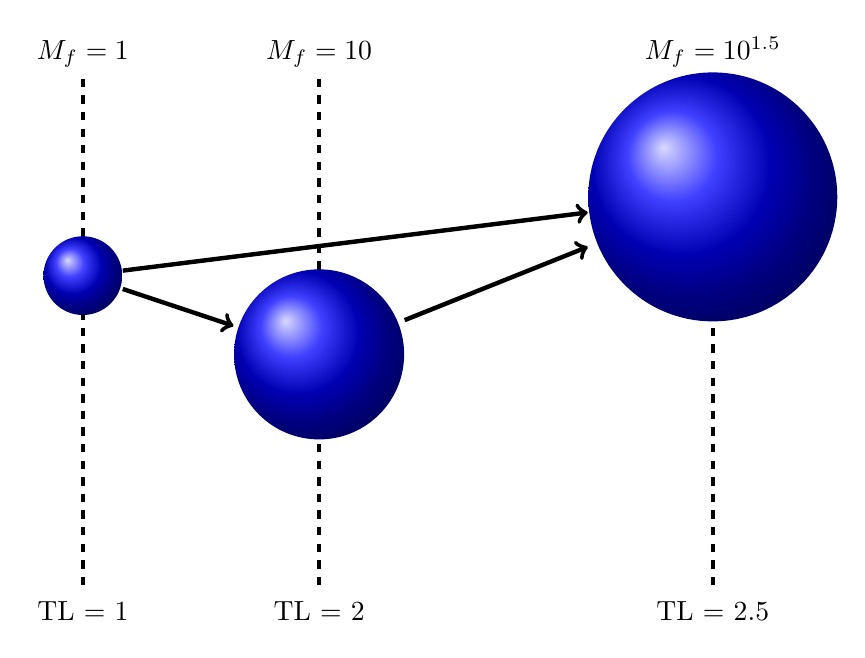
\begin{tikzpicture}
\node [inner sep = .5cm] (s1) at (0,0) {};
\node [inner sep = 1.08cm] (s2) at (3,-1) {};
%\node [inner sep = 2.313cm] (s3) at (8,1) {};
\node [inner sep = 1.581cm] (s4) at (8,1) {};
\draw[->,ultra thick] (s1) -> (s2);
%\draw[->,ultra thick] (s2) -> (s3);
\draw[->,ultra thick](s1) -> (s4);
\draw[->,ultra thick](s2) -> (s4);
\draw [ultra thick, dashed] (8,2.5) node [anchor = south]  {$M_f = 10^{1.5}$}--(8,-4) node [anchor = north] {TL = 2.5};
%\draw [ultra thick, dashed] (8,2.5) node [anchor = south]  {$M_f = 100$}--(8,-4) node [anchor = north] {TL = 3};
\draw [ultra thick, dashed] (3,2.5) node [anchor = south]  {$M_f = 10$}--(3,-4) node [anchor = north] {TL = 2};
\draw [ultra thick, dashed] (0,2.5) node [anchor = south]  {$M_f = 1$}--(0,-4) node [anchor = north] {TL = 1};
\shade [ball color=blue] (s1) circle (.5cm);
\shade [ball color=blue] (s2) circle (1.08cm);
%\shade [ball color=blue] (s3) circle (2.313cm);
\shade [ball color=blue] (s4) circle (1.581cm);
\end{tikzpicture}
}
\end{frame}

\begin{frame}
\frametitle{Consumer - Resource Body Size Ratio}
\begin{itemize}[<+->]
\item Use trophic levels:
\[
M_i=Z_f^{TL-1}
\]
\item 
\only<2>{
Maybe...?

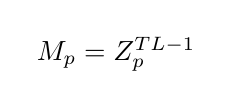
\begin{tikzpicture}
\node at (0,0) {$M_p = Z_p^{TL-1}$};
\end{tikzpicture}}

\only<3>{
Wrong!

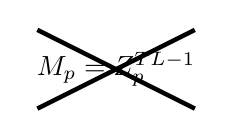
\begin{tikzpicture}
\node at (0,0) {$M_p = Z_p^{TL-1}$};
\draw [ultra thick] (-1,.5) -- (1,-.5);
\draw [ultra thick] (-1,-.5) -- (1,.5);
\end{tikzpicture}}
\end{itemize}
\end{frame}
\begin{frame}
\frametitle{Body Size Hierarchy}
$Z_f = 10$ and $Z_p = 10^{-3}$
\only<1>{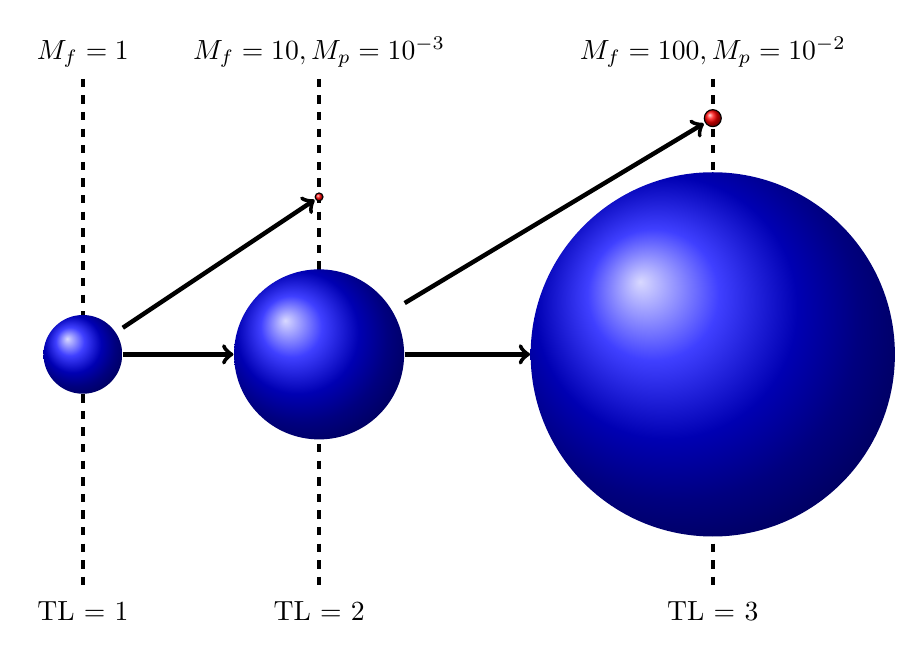
\begin{tikzpicture}
\node [inner sep = .05cm] (p1) at (3,1) {};
\node [inner sep = .108cm] (p2) at (8,2) {};
\node [inner sep = .5cm] (s1) at (0,-1) {};
\node [inner sep = 1.08cm] (s2) at (3,-1) {};
\node [inner sep = 2.313cm] (s3) at (8,-1) {};
\draw[->,ultra thick] (s1) -> (s2);
\draw[->,ultra thick] (s2) -> (s3);
\draw [ultra thick, dashed] (8,2.5) node [anchor = south]  {$M_f = 100,M_p=10^{-2}$}--(8,-4) node [anchor = north] {TL = 3};
\draw [ultra thick, dashed] (3,2.5) node [anchor = south]  {$M_f = 10,M_p=10^{-3}$}--(3,-4) node [anchor = north] {TL = 2};
\draw [ultra thick, dashed] (0,2.5) node [anchor = south]  {$M_f = 1$}--(0,-4) node [anchor = north] {TL = 1};
\draw[->,ultra thick] (s1) -> (p1);
\draw[->,ultra thick] (s2) -> (p2);
%\draw[->,dashed,thick,red] (p1) -> (p2);
%\draw[->,dashed,thick,green] (p1) -> (s3);
\shade [ball color=blue] (s1) circle (.5cm);
\shade [ball color=blue] (s2) circle (1.08cm);
\shade [ball color=blue] (s3) circle (2.313cm);
\draw [ball color=red] (p1) circle (.05cm);
\draw [ball color = red] (p2) circle (.108cm);
\end{tikzpicture}
}
\only<2>{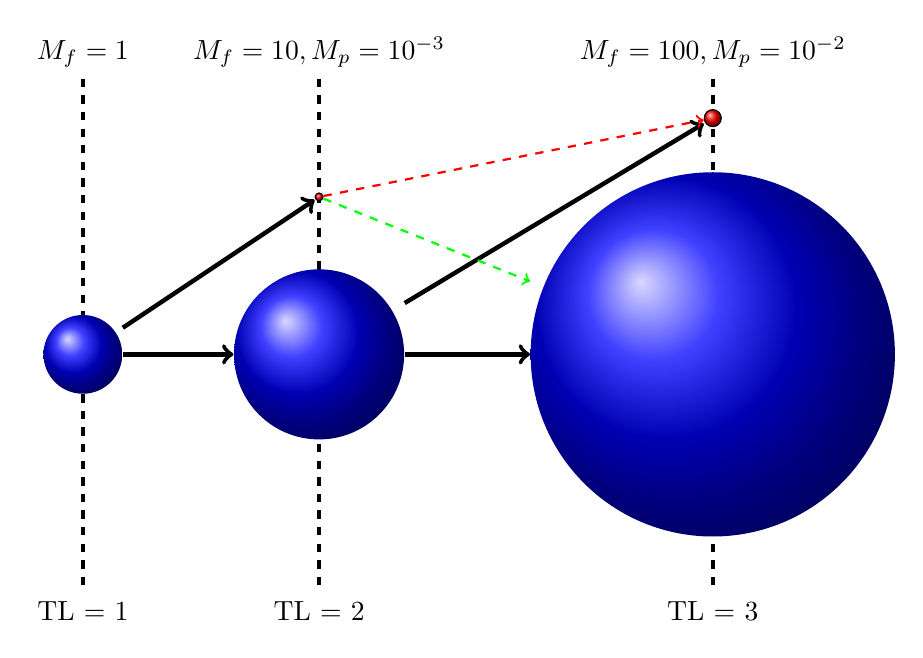
\begin{tikzpicture}
\node [inner sep = .05cm] (p1) at (3,1) {};
\node [inner sep = .108cm] (p2) at (8,2) {};
\node [inner sep = .5cm] (s1) at (0,-1) {};
\node [inner sep = 1.08cm] (s2) at (3,-1) {};
\node [inner sep = 2.313cm] (s3) at (8,-1) {};
\draw[->,ultra thick] (s1) -> (s2);
\draw[->,ultra thick] (s2) -> (s3);
\draw [ultra thick, dashed] (8,2.5) node [anchor = south]  {$M_f = 100,M_p=10^{-2}$}--(8,-4) node [anchor = north] {TL = 3};
\draw [ultra thick, dashed] (3,2.5) node [anchor = south]  {$M_f = 10,M_p=10^{-3}$}--(3,-4) node [anchor = north] {TL = 2};
\draw [ultra thick, dashed] (0,2.5) node [anchor = south]  {$M_f = 1$}--(0,-4) node [anchor = north] {TL = 1};
\draw[->,ultra thick] (s1) -> (p1);
\draw[->,ultra thick] (s2) -> (p2);
\draw[->,dashed,thick,red] (p1) -> (p2);
\draw[->,dashed,thick,green] (p1) -> (s3);
\shade [ball color=blue] (s1) circle (.5cm);
\shade [ball color=blue] (s2) circle (1.08cm);
\shade [ball color=blue] (s3) circle (2.313cm);
\draw [ball color=red] (p1) circle (.05cm);
\draw [ball color = red] (p2) circle (.108cm);
\end{tikzpicture}

}
\end{frame}

\section{Niche Model Additions}

\subsection{Proposed Models}

\subsection{Results}

\section{ATN Additions}





\subsection{Proposed Models}

\subsection{Results}

\section{Conclusions}

\section{Future Work}
\end{document}
